% ==============================================================================
% TCC - Nome do Aluno
% Capítulo 3 - Avaliação do Trabalho
% ==============================================================================
\chapter{Avaliação do Trabalho}
\label{sec-avaliacao}

\section{Testes com Dados Sintéticos}

A figura \ref{fig:compartimentos-sir-semruido} mostra o valor de 
beta ao longo do tempo.

\begin{figure}[htpb]
\centering
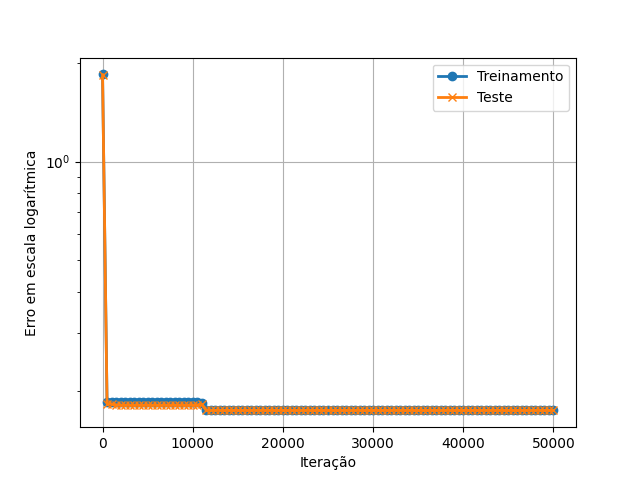
\includegraphics[width=0.6\textwidth]{figuras/loss-sir-nonoise.png}
\caption{Na primeira. Fonte: elaborada pelos autores.}
\label{fig:loss-sir-semruido}
\end{figure}


A figura \ref{fig:compartimentos-sir-semruido} mostra o valor de 
beta ao longo do tempo.

\begin{figure}[htpb]
\centering
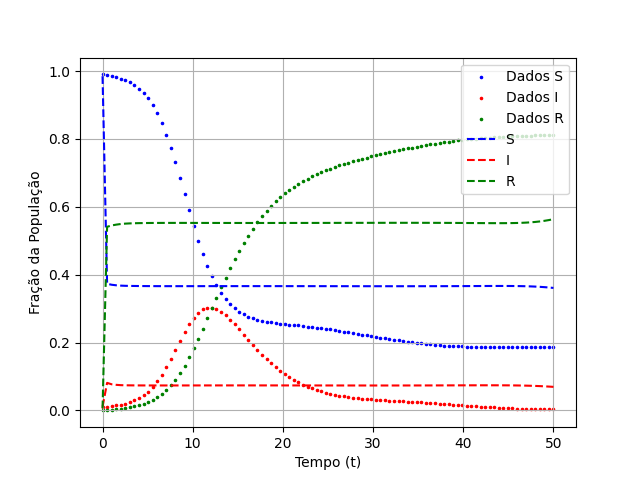
\includegraphics[width=0.6\textwidth]{figuras/predicted-compartments-sir-nonoise.png}
\caption{Na primeira. Fonte: elaborada pelos autores.}
\label{fig:compartimentos-sir-semruido}
\end{figure}

A figura \ref{fig:beta-sir-semruido} mostra o valor de beta ao longo do tempo.

\begin{figure}[htpb]
\centering
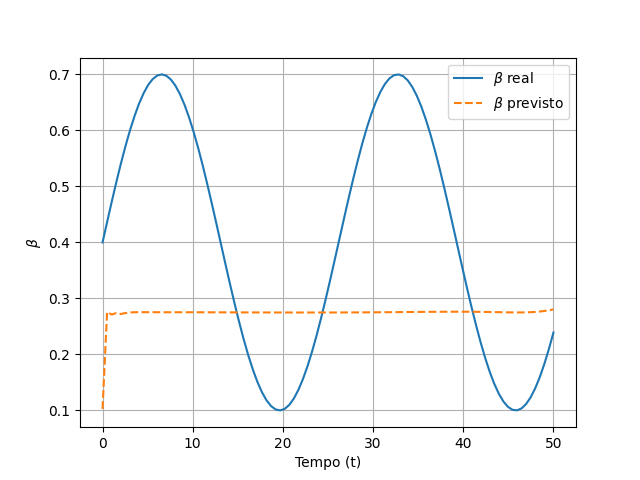
\includegraphics[width=0.6\textwidth]{figuras/predicted-beta-sir-nonoise.png}
\caption{Na primeira. Fonte: elaborada pelos autores.}
\label{fig:beta-sir-semruido}
\end{figure}


A tabela \ref{tab:metricas-dados-sinteticos} mostra os valores para 

\begin{table}[htpb]
\centering
\caption{Valores das métricas de erro (\textit{MSE}, norma $\mathcal{L}_2$ e norma $\mathcal{L}_\infty$) para as soluções aproximadas pela rede neural, em comparação com as soluções analíticas.}
\begin{tabular}{|c|c|c|c|}
\hline 
\hline 
\multirow{2}{*}{} & \multicolumn{3}{c|} {Métricas} \\ \cline{2-4} 
Compartimento & MSE & $\mathcal{L}_2$ & $\mathcal{L}_\infty$ \\ \hline
$S$ & $8{,}628 \times 10^{-6}$ & $2{,}444 \times 10^{-3}$ & $1{,}182 \times 10^{-2}$\\ \hline
$I$ & $1{,}005 \times 10^{-6}$ & $1{,}252 \times 10^{-2}$ & $4{,}81 \times 10^{-3}$\\ \hline
$R$ & $1{,}997 \times 10^{-6}$ & $4{,}913 \times 10^{-3}$ & $8{,}635 \times 10^{-3}$ \\ \hline
\hline
\end{tabular}
\label{tab:metricas-dados-sinteticos}
\end{table}


\section{Testes com Dados Ruidosos}

A figura \ref{fig:compartimentos-sir-semruido} mostra o valor de 
beta ao longo do tempo.

\begin{figure}[htpb]
\centering
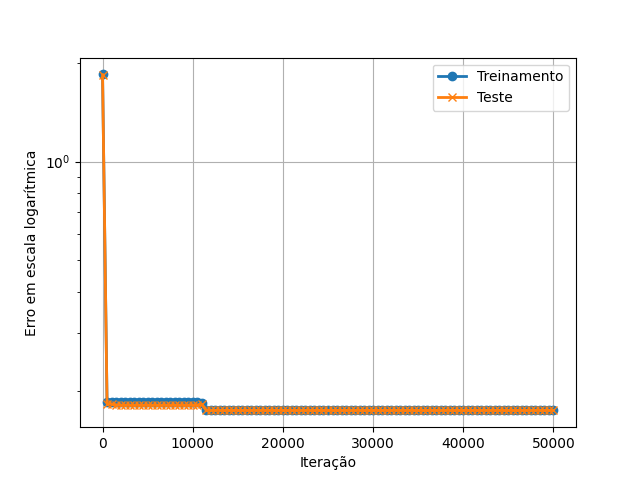
\includegraphics[width=0.6\textwidth]{figuras/loss-sir-nonoise.png}
\caption{Na primeira. Fonte: elaborada pelos autores.}
\label{fig:loss-sir-ruidoso}
\end{figure}


A figura \ref{fig:compartimentos-sir-ruidoso} mostra o valor de 
beta ao longo do tempo.

\begin{figure}[htpb]
\centering
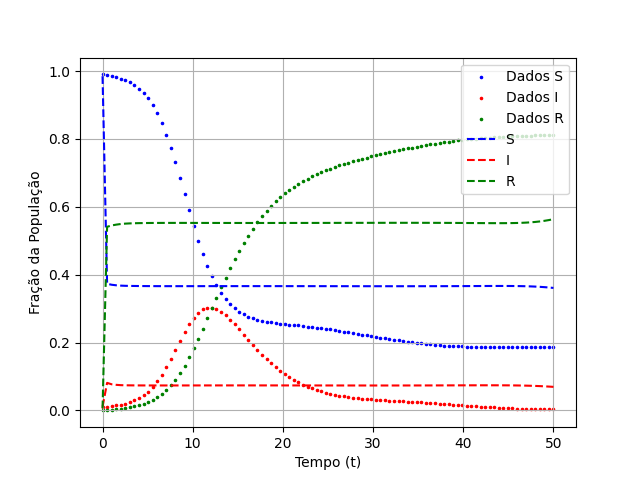
\includegraphics[width=0.6\textwidth]{figuras/predicted-compartments-sir-nonoise.png}
\caption{Na primeira. Fonte: elaborada pelos autores.}
\label{fig:compartimentos-sir-ruidoso}
\end{figure}

A figura \ref{fig:beta-sir-ruidoso} mostra o valor de beta ao longo do tempo.

\begin{figure}[htpb]
\centering
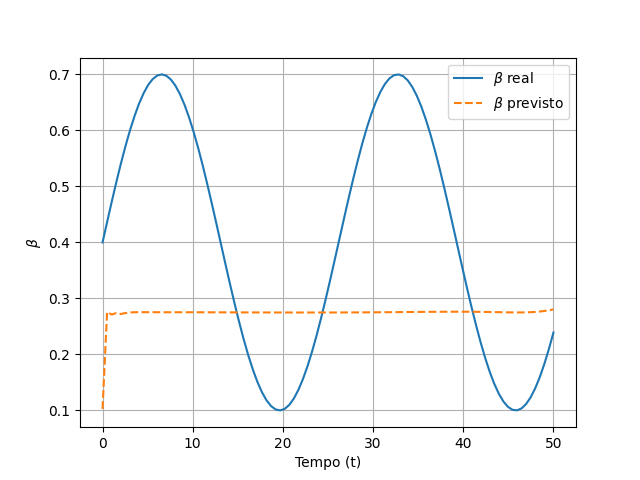
\includegraphics[width=0.6\textwidth]{figuras/predicted-beta-sir-nonoise.png}
\caption{Na primeira. Fonte: elaborada pelos autores.}
\label{fig:beta-sir-ruidoso}
\end{figure}


A tabela \ref{tab:metricas-dados-sinteticos-ruidosos} mostra os valores para 

\begin{table}[htpb]
\centering
\caption{Valores das métricas de erro (\textit{MSE}, norma $\mathcal{L}_2$ e norma $\mathcal{L}_\infty$) para as soluções aproximadas pela rede neural, em comparação com as soluções analíticas.}
\begin{tabular}{|c|c|c|c|}
\hline 
\hline 
\multirow{2}{*}{} & \multicolumn{3}{c|} {Métricas} \\ \cline{2-4} 
Compartimento & MSE & $\mathcal{L}_2$ & $\mathcal{L}_\infty$ \\ \hline
velocidade $u$ & $8{,}628 \times 10^{-6}$ & $2{,}444 \times 10^{-3}$ & $1{,}182 \times 10^{-2}$\\ \hline
velocidade $v$ & $1{,}005 \times 10^{-6}$ & $1{,}252 \times 10^{-2}$ & $4{,}81 \times 10^{-3}$\\ \hline
pressão $p$ & $1{,}997 \times 10^{-6}$ & $4{,}913 \times 10^{-3}$ & $8{,}635 \times 10^{-3}$ \\ \hline
\hline
\end{tabular}
\label{tab:metricas-dados-sinteticos-ruidosos}
\end{table}

\section{Testes com Base de Dados Reais}